
\section{Tổng quan về kiến trúc ứng dụng Android}

    \hspace*{0.8cm}Android sử dụng nhiều ngôn ngữ lập trình để phát triển ứng dụng, phổ biến nhất là Java và Kotlin. Java là ngôn ngữ truyền thống với cộng đồng lớn, trong khi Kotlin hiện đại, dễ học và được Google khuyến khích. Ngoài ra, C++, Python cũng được sử dụng trong các trường hợp đặc biệt. Việc lựa chọn ngôn ngữ phụ thuộc vào mục tiêu phát triển, loại ứng dụng và kinh nghiệm của lập trình viên. Ứng dụng Android được đóng gói dưới dạng file APK và có thể phân phối qua Google Play hoặc trực tiếp tới người dùng.

    % 1.1.
    \subsection{Các ngôn ngữ lập trình sử dụng (Java, các công nghệ đa nền tảng)}
    \renewcommand{\labelitemi}{--}    

        \hspace*{0.8cm}Ngôn ngữ lập trình Android là tập hợp các ngôn ngữ được sử dụng để viết ứng dụng cho hệ điều hành Android. Hệ điều hành này phổ biến nhất trên thế giới, với hơn 2 tỷ thiết bị đang hoạt động. Với Android Studio là môi trường phát triển tích hợp chính thức từ Google, việc lập trình ứng dụng Android trở nên dễ dàng hơn bao giờ hết. Ngôn ngữ lập trình Android không chỉ là công cụ để xây dựng các ứng dụng di động phức tạp, mà còn mở ra cơ hội cho các nhà phát triển tạo ra các trải nghiệm đa dạng, từ ứng dụng doanh nghiệp đến trò chơi giải trí độc đáo.
    
        Các ngôn ngữ lập trình phổ biến cho việc phát triển ứng dụng Android hiện nay:
        \setlength{\leftmargini}{1.5cm}
        \begin{itemize}
            \item Java: là ngôn ngữ lập trình chính cho Android từ những ngày đầu của nền tảng này. Với cộng đồng lập trình viên lớn và nhiều tài liệu hỗ trợ, Java vẫn là một trong những lựa chọn hàng đầu cho việc phát triển ứng dụng Android.\\
            Ví dụ các ứng dụng đang sử dụng Java : Facebook, WhatApps,…
            \item Kotlin: là ngôn ngữ có độ phổ biến ngày càng tăng cho việc phát triển ứng dụng Android. Kotlin cung cấp các tính năng hiện đại và làm cho việc viết mã dễ dàng hơn so với Java. Với sự ủng hộ mạnh mẽ từ Google, Kotlin đang trở thành ngôn ngữ lập trình được ưa chuộng nhất cho Android.\\
            Ví dụ các ứng dụng đang sử dụng Kotlin : Pinterest, Trello,…
            \item Dart: là ngôn ngữ lập trình được sử dụng với framework Flutter – một công nghệ do Google phát triển để xây dựng ứng dụng đa nền tảng (Android, iOS, web, desktop). Dart cho phép lập trình viên viết một lần và triển khai trên nhiều nền tảng, với hiệu suất cao và giao diện người dùng đẹp mắt.\\
            Ví dụ các ứng dụng đang sử dụng Dart (với Flutter): Google Ads, Alibaba, Reflectly,…
        \end{itemize}

        Việc lựa chọn ngôn ngữ lập trình nào để phát triển ứng dụng Android phụ thuộc vào nhiều yếu tố, bao gồm:
        \setlength{\leftmargini}{1.5cm}
        \begin{itemize}
            \item Kinh nghiệm và sở thích của lập trình viên: Nếu bạn đã có kinh nghiệm với Java hoặc Kotlin, bạn có thể sử dụng ngôn ngữ đó để phát triển ứng dụng Android. Nếu bạn mới bắt đầu học lập trình Android, Kotlin có thể là lựa chọn tốt hơn vì nó dễ học hơn Java.
            \item Loại ứng dụng bạn muốn phát triển: Một số ngôn ngữ lập trình phù hợp hơn với các loại ứng dụng nhất định. Ví dụ, C++ là lựa chọn tốt cho các trò chơi, trong khi Python là lựa chọn tốt cho các ứng dụng đơn giản.
            \item Mục tiêu phát triển: Phát triển nhanh(Python, Kotlin), hiệu suất cao(C++), Bảo trì dễ dàng(Java, Kotlin).
            \item Xu hướng thị trường: Kotlin là ngôn ngữ được Google khuyến khích sử dụng cho phát triển ứng dụng Android và đang dần trở nên phổ biến nhờ cú pháp hiện đại và khả năng tương thích tốt. Bên cạnh đó Java vẫn giữ vị trí là ngôn ngữ phổ biến nhất cho Android, tuy nhiên đang dần được thay thế bởi Kotlin trong nhiều dự án mới. Tiếp theo, C++ thường được sử dụng cho các ứng dụng đòi hỏi hiệu suất cao, như game hoặc xử lý đồ họa, nhưng không phổ biến bằng Java hay Kotlin. Trong khi đó, Python ít được sử dụng cho Android do hạn chế về hiệu suất và hỗ trợ nền tảng, tuy nhiên vẫn có thể phù hợp với các ứng dụng đơn giản hoặc phục vụ mục đích học tập, thử nghiệm.        
            \item Hỗ trợ từ cộng đồng: Các ngôn ngữ lập trình phổ biến hơn có cộng đồng hỗ trợ lớn hơn, giúp bạn dễ dàng tìm kiếm trợ giúp khi gặp khó khăn.   
        \end{itemize}

    % 1.2.
    \subsection{File APK và quá trình đưa ứng dụng lên Google Play, App Store}
    \renewcommand{\labelitemi}{--}
        \hspace*{0.8cm}APK (Android Package) là định dạng tập tin được sử dụng để phân phối và cài đặt ứng dụng trên hệ điều hành Android, có đuôi mở rộng .apk, tương tự như .exe trong Windows hoặc .ipa trong IOS. Là gói nén chứa toàn bộ tài nguyên và mã thực thi của ứng dụng.\\
        Cấu trúc bên trong một file APK
        \begin{figure}[H] 
            \centering
            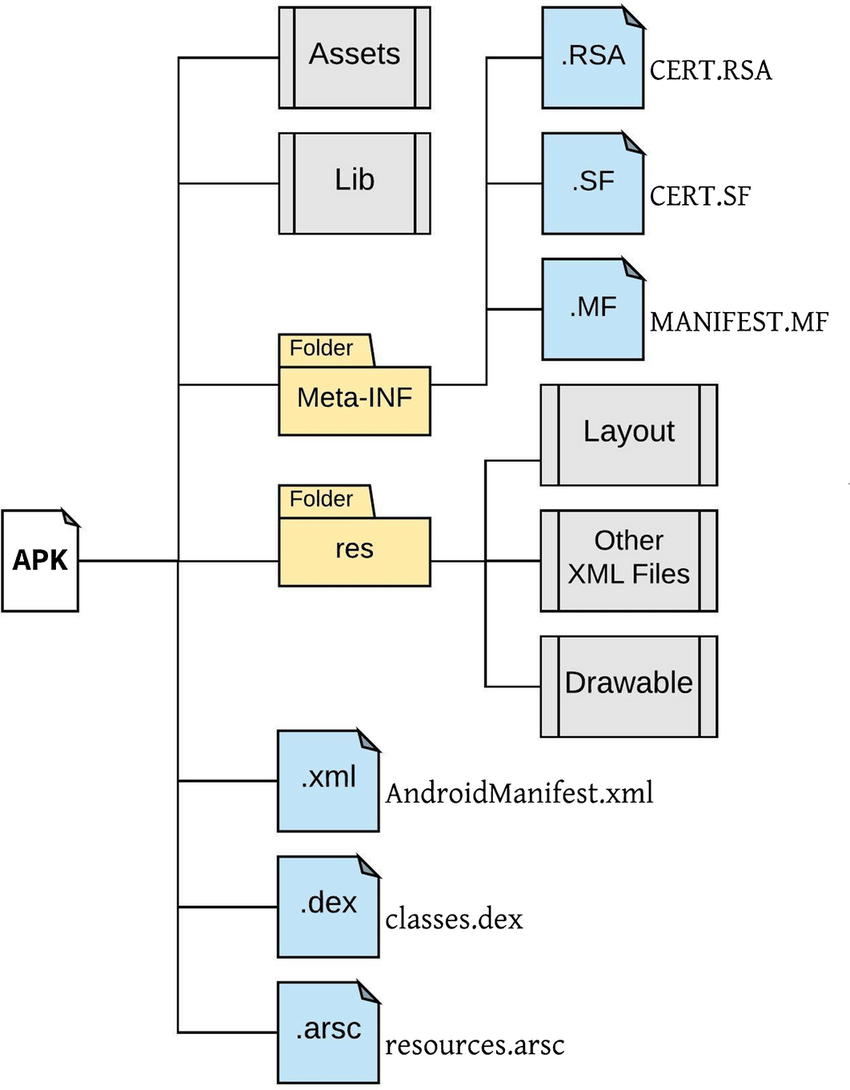
\includegraphics[width=0.5\textwidth]{images/apk.png}
            \caption{Cấu trúc file APK}
            \label{fig:android}
        \end{figure}
        
        \begin{table}[H]
            \centering
            \renewcommand{\arraystretch}{1.5}
            \begin{tabular}{|l|p{11cm}|}
                \hline
                \textbf{Thành phần} & \textbf{Mô tả} \\
                \hline
                \texttt{AndroidManifest.xml} & Chứa thông tin cấu hình ứng dụng: tên gói, phiên bản, các quyền truy cập, khai báo thành phần như Activity, Service, Receiver \cite{AndroidManifest.xml}... \\
                \hline
                \texttt{classes.dex} & Chứa mã bytecode đã được biên dịch từ mã nguồn Java hoặc Kotlin. Đây là phần chính được thực thi trong máy ảo Dalvik hoặc ART. \\
                \hline
                \texttt{resources.arsc} & Tập hợp các tài nguyên đã được biên dịch như chuỗi ký tự (string), style, màu sắc và các giá trị được lưu trong XML. \\
                \hline
                \texttt{res/} & Thư mục chứa các tài nguyên chưa biên dịch như hình ảnh, layout XML, drawable, v.v. \\
                \hline
                \texttt{lib/} & Thư mục chứa các thư viện native (viết bằng C/C++) tương ứng với từng kiến trúc CPU (như ARM, x86...). \\
                \hline
                \texttt{META-INF/} & Lưu trữ các tệp liên quan đến chứng chỉ số, thông tin chữ ký APK để xác thực và bảo vệ toàn vẹn nội dung. \\
                \hline
                \texttt{assets/} & Chứa các tài nguyên thô (raw) do lập trình viên thêm vào, có thể truy cập qua `AssetManager`. \\
                \hline
            \end{tabular}
            \caption{Cấu trúc các thành phần bên trong file APK}
            \label{table:apk-structure}
            \end{table}            
    
        Quy trình khi đưa ứng dụng lên Google Play: Build APK, từ mã nguồn Android (bằng Android Studio), tạo ra file .apk. Ký số (Signing), ứng dụng được ký bằng private key để xác thực nguồn gốc. Upload lên Google Play, Google kiểm tra, và nếu muốn, có thể dùng App Signing by Google Play, là dịch vụ Google giữ private key. Phân phối và cài đặt, người dùng tải về và cài đặt ứng dụng trực tiếp từ APK.\\

        Tóm lại APK là đơn vị triển khai duy nhất trên Android, có thể chia sẻ trực tiếp (qua web, Bluetooth, email…) mà không cần qua Play Store, dễ dàng trích xuất hoặc phân tích để debug hoặc reverse engineering (nên phải cẩn thận bảo vệ mã nguồn).
